% !TEX TS-program = sage
\documentclass{amsart}
\usepackage[landscape,top=.5in,bottom=.5in,right=.25in,left=.25in,headsep=.25in,footskip=0.35in,centering]{geometry}
\usepackage{array} % for better arrays (eg matrices) in maths
\usepackage{paralist} % very flexible & customisable lists (eg. enumerate/itemize, etc.)
\usepackage{subfig} % make it possible to include more than one captioned figure/table in a single float
\usepackage{booktabs} % for much better looking tables
\usepackage{verbatim} % adds environment for commenting out blocks of text & for better verbatim
\usepackage{tikz} % adds environment for commenting out blocks of text & for better verbatim
\usepackage{sagetex} % adds environment for commenting out blocks of text & for better verbatim
\usepackage{multicol}
\usepackage{cmbright}
% 
\usepackage{fancyhdr}
\pagestyle{fancyplain} 
\fancyhead[co]{\textbf{\huge{Trigonometry}}}
\fancyfoot[le]{\tiny{Prepared using \LaTeX}}
\fancyfoot[re]{\textcopyright\tiny{\today Philip R. Huffman}}
\fancyfoot[c]{}

\begin{document}
\renewcommand{\headrulewidth}{0pt}


\renewcommand{\headrulewidth}{0pt}
\begin{multicols}{2}
    \subsection*{Essential Definitions:}\ \vspace{6pt} \\
    The Unit Circle: $x^2+y^2=1$\\
%    
    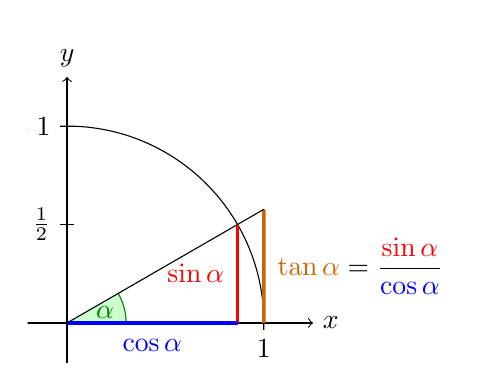
\begin{tikzpicture} [scale=2.5,line cap=round 
% Styles 
axes/.style=,
important line/.style={very thick}, 
information text/.style={rounded corners,fill=red!10,inner sep=1ex}]
% Local definitions
\def\costhirty{0.8660256}
% Colors
\colorlet{anglecolor}{green!50!black} 
\colorlet{sincolor}{red} 
\colorlet{tancolor}{orange!80!black} 
\colorlet{coscolor}{blue}
\begin{scope}
\clip (-0.2,-0.2) rectangle (2,1.5);
\draw (0,0) circle (1cm);
\begin{scope}%[axes] 
    \draw[<->] (-1.25,0) -- (1.25,0) node[right] {$x$} coordinate(x axis); 
    \draw[<->] (0,-1.25) -- (0,1.25) node[above] {$y$} coordinate(y axis);
    \foreach \x/\xtext in {-1, -.5/-\frac{1}{2}, 1} 
        \draw[xshift=\x cm] (0pt,1pt) -- (0pt,-1pt) node[below,fill=white] {$\xtext$};
    \foreach \y/\ytext in {-1, -.5/-\frac{1}{2}, .5/\frac{1}{2}, 1} 
        \draw[yshift=\y cm] (1pt,0pt) -- (-1pt,0pt) node[left,fill=white] {$\ytext$};
\end{scope}
\filldraw[fill=green!20,draw=anglecolor] (0,0) -- (3mm,0pt) arc(0:30:3mm); \draw (15:2mm) node[anglecolor] {$\alpha$};
\draw[important line,sincolor] (30:1cm) -- node[left=1pt,fill=white] {$\sin \alpha$} (30:1cm |- x axis);
\draw[important line,coscolor] (30:1cm |- x axis) -- node[below=2pt,fill=white] {$\cos \alpha$} (0,0);
\draw[important line,tancolor] (1,0) -- node[right=1pt,fill=white] 
{ $\displaystyle \tan \alpha \color{black}= \frac{{\color{sincolor}\sin \alpha}}{\color{coscolor}\cos \alpha}$} 
(intersection of 0,0--30:1cm and 1,0--1,1) coordinate (t);
\draw (0,0) -- (t);
(-0.2,-0.2) rectangle (2,1.5);
\end{scope}
\end{tikzpicture}
\vspace{3pt}

        \begin{tabular}{|lll|lll|}\hline
            $\sin\alpha$  &= $y$                &$\Rightarrow\frac{opposite}{hypotenuse}$ & $\cos\alpha$ & $=x$                 & $\Rightarrow\frac{adjacent}{hypotenuse}$\\
            $\tan\alpha$  &= $\frac{y}{x}$ &$\Rightarrow\frac{opposite}{adjacent}$      & $\csc\alpha$ & $=\frac{1}{y}$  & $\Rightarrow\frac{hypotenuse}{opposite}$\\
            $\sec\alpha$ &= $\frac{1}{x}$ &$\Rightarrow\frac{hypotenuse}{adjacent}$ & $\cot\alpha$ & $=\frac{x}{y}$  & $\Rightarrow\frac{adjacent}{opposite}$\\ \hline
        \end{tabular}
        \vspace{4pt}
    
    \begin{Small}
	Where opposite, adjacent and hypotenuse are three sides of a right triangle.
        Opposite is the length of the side opposite $\alpha$. Adjacent is the length of the side adjacent to $\alpha$.
        Hypotenuse is the length of the longest side.\vspace{4pt}
    \end{Small}
    
    \setlength{\extrarowheight}{4pt}
    \begin{tabular}[c]{|c|ccccccc|} \hline
        $\theta$&0&$\frac{\pi}{6}$&$\frac{\pi}{4}$&$\frac{\pi}{3}$&$\frac{\pi}{2}$&$\pi$&$\frac{3\pi}{2}$\\ \hline  
        $\sin\theta$&0&$\frac{1}{2}$&$\frac{\sqrt{2}}{2}$&$\frac{\sqrt{3}}{2}$&1&0&-1\\
        $\cos\theta$&1&$\frac{\sqrt{3}}{2}$&$\frac{\sqrt{2}}{2}$&$\frac{1}{2}$&0&-1&0\\
        $\tan\theta$&0&$\frac{\sqrt{3}}{3_{}}$&1&$\sqrt{3}$&Undefined&0&Undefined\\ \hline
    \end{tabular}
    
    \subsection*{Use radians for all calculations} $\pi =180^{\circ}$
    \subsection*{Linear Speed} $v=\frac{s}{t}$\\$\theta =\frac {s}{r}\Leftrightarrow r\theta = s\Leftrightarrow\frac{s}{t}=\frac{r\theta}{t}$
    \subsection*{Angular Speed} $\omega =\frac{\theta }{t}$
    \subsection*{Area of a Sector of a Circle} $A=\frac{r^2\theta }{2}$
    \subsection*{Periodic Functions} $f(t+c)=f(t)$
    \subsection*{Even functions} $\cos$ and $\sec$  (y-axis symmetry).
    \subsection*{Odd functions} $\sin$ and $\csc$ (origin symmetry).
    \subsection*{Reference Angle}
     Let $\theta$ be an angle in standard position. Its reference angle is the acute angel $\theta '$ formed by the terminal side of
    $\theta$ and the horizontal axis.
    \subsection*{Pythagorean Identities:}
    \[\sin^2\alpha + \cos^2\alpha = 1\qquad\tan^2\alpha +1 = \sec^2\alpha\qquad\cot^2\alpha +1 = \csc^2\alpha\]
    \subsection*{Cofunction Identities:}
    \begin{center}
    \begin{tabular}[c]{ll}
       $\sin\left(\frac{\pi}{2}-u\right)=\cos u$ & $\cos\left(\frac{\pi}{2}-u\right)=\sin u$ \\
       $\tan\left(\frac{\pi}{2}-u\right)=\cot u$ & $\cot\left(\frac{\pi}{2}-u\right)=\tan u$ \\
       $\sec\left(\frac{\pi}{2}-u\right)=\csc u$ & $\csc\left(\frac{\pi}{2}-u\right)=\sec u$
    \end{tabular}
    \end{center}
    \subsection*{Even/Odd identities:}
    \begin{center}
    \begin{tabular}[c]{lll}
        $\sin(-u)=-\sin u$ & $\cos(-u)=\cos u$ & $\tan(-u)=-\tan u$\\
        $\csc(-u)=-\csc u$ & $\sec(-u)=\sec u$ & $\cot(-u)=-\cot u$
    \end{tabular}
    \end{center}
    \subsection*{Graphs}$y=a\sin(bx-c)$ and $y=a\cos(bx-c), b>0)$
    \begin{enumerate}
        \item Amplitude $=|a|$
        \item Period $=\frac{2\pi}{b}$
        \item Endpoints for one period: $\left[\frac{c}{b},\frac{2\pi +c}{b}\right)$
    \end{enumerate}
    \subsection*{Simple Harmonic Motion}$d=a\sin\omega t\text{ or }d=a\cos\omega t$\hfill \\
    Where $a$ and $\omega$ are real numbers and $\omega > 0$.\\
    Frequency: $\frac{\omega}{2\pi}$, Period: $\frac{2\pi}{\omega}$
    \subsection*{ Law of Sines:}
    $\dfrac{a}{\sin A}=\dfrac{b}{\sin B}=\dfrac{c}{\sin C}$\medskip\\
    SSA (The Ambiguous Case) \hskip 6pt Given $a, b, A.\quad (h=b\sin A)$
    \begin{center}
    \begin{small}\begin{tabular}[c]{|l|cccccc|}\hline
        \textit{A is}&acute&acute&acute&acute&obtuse&obtuse\\\hline
        \textit{Condition}&$a<h$&$a=h$&$a>b$&$h<a<b$&$a<b$&$a>b$\\
        \textit{\# Possible}&0&1&1&2&0&1\\\hline
    \end{tabular}\end{small}
    \end{center}
    \subsection*{Area of an Oblique Triangle:}$\frac{bc\sin A}{2}$ or $\frac{ab\sin C}{2}$ or $\frac{ac\sin B}{2}$
    \subsection*{Heron's Formula:} $A=\sqrt{s(s-a)(s-b)(s-c)}\;,\quad s=\frac{a+b+c}{2}$
    \subsection*{Law of Cosines:}
    \begin{center}
    \begin{tabular}[c]{cc}
        \large{\textit{Standard Form}} &\large{\textit{Alternate Form}}\\
        $a=\sqrt{b^2+c^2-2bc\cos A}$&$\cos A=\frac{b^2+c^2-a^2}{2bc}$\\
        $b=\sqrt{a^2+c^2-2ac\cos B}$&$\cos B=\frac{a^2+c^2-b^2}{2ac}$\\
        $c=\sqrt{a^2+b^2-2ab\cos C}$&$\cos C=\frac{a^2+b^2-c^2}{2ab}$
    \end{tabular}
    \end{center}
    \subsection*{ Sum and Difference Formulae:}
    \begin{align*}
    \sin(u\pm v)&=\sin u\cos v\pm\cos u\sin v\\
    \cos(u\pm v)&=\cos u\cos v\mp\sin u\sin v\\
    \tan(u\pm v)&=\frac{\tan u\pm \tan v}{1\mp\tan u\tan v}
    \end{align*}
    \subsection*{Double-Angle Formulae:}
    \begin{align*}
    \sin 2u&=2\sin u\cos u\\\cos 2u&=\cos^2u-\sin^2u=1-2\sin^2u=2\cos^2u-1\\\tan 2u&=\frac{2\tan u}{1-\tan^2u}
    \end{align*}
    \subsection*{Half-Angle Formulae:}
    \begin{align*}
    \sin\frac{u}{2}&=\pm\sqrt{\frac{1-\cos u}{2}}\\
    \cos\frac{u}{2}&=\pm\sqrt{\frac{1+\cos u}{2}}\\
    \tan\frac{u}{2}&=\frac{1-\cos u}{\sin u}=\frac{\sin u}{1+\cos u}
    \end{align*}
    \subsection*{Power Reducing Formulae:}
    \begin{align*}
    sin^2u&=\frac{1-\cos 2u}{2}\\\cos^2u&=\frac{1+\cos 2u}{2}\\\tan^2u&=\frac{1-\cos 2u}{1+\cos 2u}
    \end{align*}
    \subsection*{Sum-to-Product Formulae:}
    \begin{align*}
    \sin u+\sin v&=2\sin\left(\frac{u+v}{2}\right)\cos\left(\frac{u-v}{2}\right)\\
    \sin u-\sin v&=2\cos\left(\frac{u+v}{2}\right)\sin\left(\frac{u-v}{2}\right)\\
    \cos u+\cos v&=2\cos\left(\frac{u+v}{2}\right)\cos\left(\frac{u-v}{2}\right)\\
    \cos u-\cos v&=-2\sin\left(\frac{u+v}{2}\right)\sin\left(\frac{u-v}{2}\right)
    \end{align*}
    \subsection*{Product-to-Sum Formulae:}
    \begin{align*}
    \sin u\sin v&=\frac{\cos(u-v)-\cos(u+v)}{2}\\
    \cos u\cos v&=\frac{\cos(u-v)+\cos(u+v)}{2}\\
    \sin u\cos v&=\frac{\sin(u+v)+\sin(u-v)}{2}\\
    \cos u\sin v&=\frac{\sin(u+v)-\sin(u-v)}{2}
    \end{align*}
    \subsection*{Vectors:}
    \begin{enumerate}
        \item $\overrightarrow{PQ}=\langle q_1-p_1,q_2-p_2\rangle=\langle v_1,v_2\rangle=v$\hfill Component Form
        \item $\Vert\overrightarrow{PQ}\Vert=\sqrt{(q_1-p_1)^2+(q_2-p_2)^2}$\hfill Magnitude
    \end{enumerate}
    \subsection*{Dot Product Properties:}
    \begin{enumerate}
        \item $u\cdot v=u_1v_1+u_2v_2$\hfill Dot Product
        \item $0\cdot u=0$
        \item $u\cdot u=\Vert u\Vert^2$
        \item $u\cdot v=v\cdot u$
        \item $u\cdot (v+w)=u\cdot v+u\cdot w$
        \item $(cu)\cdot v=c(u\cdot v)=u\cdot cv$
        \item $u\cdot v=0$\hfill Orthogonal Vectors
        \item $\cos\theta = \frac{u\cdot v}{\Vert u\Vert\Vert v\Vert}$\hfill Angle between Two Vectors
%Vectors
        \item $proj_vu=\left(\frac{u\cdot v}{\Vert v\Vert^2}\right)v$\hfill Projection of $u$ onto $v$
    \end{enumerate}
    \subsection*{ Work ($F$ is constant):}
    \begin{enumerate}
        \item $W=\Vert F\cdot\overrightarrow{PQ}\Vert$\hfill Dot Product Form
        \item $W=\Vert proj_{\overrightarrow{PQ}}F\Vert\Vert\overrightarrow{PQ}\Vert$\hfill Projection Form
    \end{enumerate}
    \subsection*{Demoivre's Theorem:}
    If $n$ is a positive integer, Then
    \begin{align*}
    \left[r\left(\cos\theta+i\sin\theta\right) \right]^n&=r^n\left(\cos n\theta+i\sin n\theta\right) \\ 
    \text{ Example: Find } \sqrt[3]{8i}\qquad\left(n=3,r=2\right)\\ 
    0+8i&=2^{3}\left(\cos\frac{\pi}{2}+i\sin\frac{\pi}{2}\right) \\
    z^3=8i\Leftrightarrow 2^3(\cos3\theta+i\sin3\theta)&=2^{3}\left(\cos\dfrac{\pi}{2}+i\sin\dfrac{\pi}{2}\right) \\ 
    3\theta&=\dfrac{\pi}{2}+2\pi n\\
    \theta&=\dfrac{\pi}{6}+\dfrac{2\pi n}{3} \\
    r=2,\;2\left(\cos\dfrac{\pi}{6}+i\sin\dfrac{\pi}{6}\right)&=\boxed{\sqrt{3}+i} \\
     2\left(\cos\dfrac{5\pi}{6}+i\sin\dfrac{5\pi}{6}\right)&=\boxed{-\sqrt{3}+i} \\
     2\left(\cos\dfrac{3\pi}{2}+i\sin\dfrac{3\pi}{2}\right)&=\boxed{-2i}
\end{align*}
\end{multicols}
\end{document}
